\documentclass{plantilla-manual-usuario}

\autor{PRYADES Soluciones Informáticas SL}
\proyecto{Teleradiología en la Nube}
\logotipo{images/imedig-logo.jpg}
\title{Manual de Usuario}
\company{images/pryades-logo.png}
\date{02/09/2015}

\begin{document}

\frontmatter

\maketitle

\newpage

\tableofcontents

\mainmatter
\clearpage

\section{Introducción}

La teleradiología es una necesidad para centros médicos que no disponen de los servicios de un radiólogo pero que disponen de tecnología para la adquisición de imágenes médicas. Cuando se necesita de este tipo de servicio especializado, el procedimiento usual es el de remitir al paciente a un hospital con los consecuentes gastos, molestias y demoras para el paciente en obtener su diagnóstico, así como la congestión de estos servicios en el hospital.

IMEDIG Cloud es una aplicación Web en la Nube que facilita este proceso aprovechando las redes de telecomunicaciones disponibles sin necesidad de desplazamientos ni demoras excesivas. Este documento está dirigido a imagenólogos y médicos que utilizarán IMEDIG para la teleradiología.

La elaboración de un informe radiológico con IMEDIG está compuesta por las siguientes etapas: 

\begin{itemize}
\item Solicitud de informe.
\item Escritura de informe.
\item Aprobación de informe.
\item Consulta de informe.
\end{itemize}

Cada una de estas etapas se explicarán en detalle a continuación. 


\section{Inicio de aplicación}

La interfaz de IMEDIG se inicia introduciendo en un navegador Web (compatibles Chrome, Safari, Firefox, IE 9+) la dirección http://www.imedig.com/cloud.

La ventana inicial de la aplicación mostrará un formulario de Autentificación (ver figura \referencia{figuraLogin}) en el que el usuario deberá identificarse con su identificador y contraseña. 

\figura{0.35}{images/login.png}{Autenticación de usuario}{figuraLogin}{}

En caso de que haya olvidado la contraseña de acceso al sistema el usuario puede utilizar la opción ”¿Ha olvidado la contraseña?” que aparece en la parte inferior del formulario. Allí introduce su dirección de correo electrónico o nombre de usuario y presionando el botón ”Enviar contraseña por email” recibirá una notificación por correo electrónico con una contraseña nueva. Al acceder usando la contraseña nueva el sistema le mostrará una ventana para que establezca su propia contraseña de acceso.

Cuando el usuario y contraseña introducidos hayan sido validados se mostrará una lista de centros radiológicos a los que el usuario tiene acceso para consultar imágenes e informes. Cada centro estará representado mediante un cuadro con el nombre y logotipo del Centro (figura \referencia{figuraListaDeCentros}).

\figura{1}{images/lista-de-centros.png}{Lista de centros}{figuraListaDeCentros}{}

Al iniciar la aplicación y durante un breve tiempo el fondo de los recuadros de centro se muestran de color amarillo indicando que se está chequeando la disponibilidad de la conexión con el centro. Después de unos segundos este color de fondo cambia para indicar que la conexión está disponible o no. Así, si el fondo del cuadro es rojo, no hay conexión habilitada con el centro correspondiente. El color verde indica disponibilidad de conexión (ver figura \referencia{figuraCentroConectado}). Adicionalmente un color azúl indica que hay nuevos informes solicitados, por aprobar o aprobados para dicho centro. 

\figura{0.3}{images/centro-disponible.png}{Centro disponible }{figuraCentroConectado}{}

Al hacer clic con el ratón sobre el recuadro de un centro con la conexión habilitada se abre una ventana como la de la figura \referencia{figuraVistaInterfazImagenes}. Esta ventana contiene la interfaz de la aplicación para consultar imágenes y/o solicitar informes (consultar detalles de esta interfaz en el epígrafe \referencia{sectionInterfazdeImagenes}).

\figura{1}{images/vista-interfaz.png}{Interfaz para consultar imágenes y/o solicitar informes}{figuraVistaInterfazImagenes}{}

Para utilizar una versión demostrativa de la aplicación introduzca los siguientes datos en la ventana de autentificación:

\begin{itemize}
\item Usuario: demo
\item Contraseña: demo 
\end{itemize}

En la parte superior derecha de la ventana principal aparecen iconos con las siguientes fucionalidades:

\begin{itemize}
\item 
\includegraphics[scale=0.5]{images/boton-ayuda.png} Ayuda: Muestra una nueva ventana en la que se muestra este manual en formato PDF.
\item 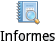
\includegraphics[scale=0.5]{images/boton-informes.png} Informes: Accede a la interfaz de Gestión de Informes (ver sección \referencia{sectionGestiondeInformes}).
\item 
\includegraphics[scale=0.5]{images/exit.png} Salir: Cierra la sesión de usuario y sale de la aplicación Web.
\end{itemize}

\section{Solicitud de informe}\label{subsectionSolicitarInforme}

Para solicitar un informe, el médico referidor o personal administrativo designado, presionará el botón izquierdo del ratón sobre el cuadro del centro correspondiente para abrir la interfaz de gestión de imágenes correspondiente a dicho centro como se explica en el epígrafe \referencia{sectionInterfazdeImagenes}.

Una vez seleccionado el estudio deberá abrir una imagen representativa del estudio para incluir en la solicitud y hacer clic con el ratón sobre el botón  ”Solicitar informe” que está en la parte inferior de la ventana tal como se muestra en la figura \referencia{figuraVistaInterfazImagenes}. Los detalles de cómo encontrar y abrir una imagen en la interfaz de consulta pueden consultarse en el epígrafe \referencia{sectionAbrir}.

Al presionar el botón ”Solicitar informe” se abrirá una ventana que permite escribir los detalles referentes a la solicitud (ver figura \referencia{figuraNuevoInforme}).

\figura{0.8}{images/nuevo-informe.png}{Solicitar nuevo informe}{figuraNuevoInforme}{}

En la parte media de la ventana hay una región dedicada a la edición del contenido de la solicitud del informe. En ella debe explicarse la historia clínica del paciente que es relevante para facilitar el diagnóstico por parte del radiólogo.

Debajo de la región de edición del contenido del informe se selecciona (opcionalmente) el médico que solicita el informe. Además, un cuadro de chequeo permite restringir el personal que tendrá acceso al informe. Si se marca el cuadro de ”Acceso solo al referidor” solamente el médico seleccionado como referidor y los radiólogos podrán ver el contenido del mismo. Esta opción sólo debe usarse en casos especiales que así lo requieran.

Cuando se haya completado la solicitud debe presionarse el botón ”Solicitar” para añadirla a la lista de informes \italics{Solicitados}.

\section{Interfaz de Gestión de Informes}\label{sectionGestiondeInformes}

Haciendo clic con el ratón sobre el botón 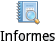
\includegraphics[scale=0.6]{images/boton-informes.png} incluido en la barra superior de IMEDIG aparece una ventana como la de la figura \referencia{figuraGestionInformes}. Esta ventana incluye opciones con las que se se pueden cribar los informes que se listan en la tabla que está en la parte media de la ventana. Además, contiene botones que permiten visualizar, aprobar, modificar, o eliminar informes una vez hayan sido localizados.

\figura{1}{images/gestion-informe.png}{Ventana Gestión de Informes}{figuraGestionInformes}{}

En la parte superior de la interfaz hay entradas que permiten fijar criterios de búsqueda para filtrar los informes que se muestran en la tabla. Los informes registrados contienen estos datos según han sido rellenados al hacer la solicitud o al modificarlos (su significado está descrito en el epígrafe \referencia{subsectionModificarInforme}). Introduzca los valores correspondientes a los informes que desea encontrar y presione el botón 
\includegraphics[scale=0.4]{images/buscar-informes.png} para obtener una lista reducida en la tabla y simplificar la búsqueda. Los criterios que pueden aplicarse en la búsqueda son:

\begin{itemize}
\item Fecha: Búsqueda por fecha.
\item Estado: Búsqueda por el estado de aprobación del informe. Para listar todos los informes seleccione \italics{Todos}.
\item Refiere: Búsqueda por el médico que refirió el estudio del que se hizo el informe.
\item Informa: Búsqueda por el radiólogo que hizo el informe.
\item Centro: Búsqueda por el centro al que pertenece el informe.
\item Modalidad: Búsqueda por modalidad de la imagen incluida en el informe.
\item Estudio: Búsqueda por identificador del estudio del cual se hizo el informe.
\item Paciente:  Búsqueda por identificador o nombre de paciente.
\item Diagnóstico: Búsqueda por código de diagnóstico.
\item Palabras clave: Búsqueda por palabras clave del informe.
\end{itemize}

Seleccione el informe que le interesa de la lista de resultados que aparece en la tabla y presione el botón correspondiente a la acción que desea efectuar sobre él. En la parte inferior de la figura \referencia{figuraGestionInformes} aparecen los botones con las acciones disponibles. Ellas serán descritas en los epígrafes subsiguientes y son:

\begin{itemize}
\item Mostrar
\item Modificar
\item Eliminar
\item Aprobar
\end{itemize}

Los informes que están en estado \italics{Aprobado} no pueden ser modificados, ni eliminados. Tampoco es posible aprobarlos otra vez. Por eso, si el informe que se selecciona en la tabla tiene el estado \italics{Aprobado}, la única opción que puede aplicarse sobre él es ”Mostrar”.

\subsection{Mostrar informe}\label{subsectionMostrarInforme}
Esta opción se activa si se selecciona uno de los informes de los resultados que aparecen en la tabla de la figura \referencia{figuraGestionInformes} y después se presiona el botón ”Mostrar”. Permite visualizar un archivo en formato PDF con el contenido del informe. Aparecerá la ventana de la figura \referencia{figuraMostrarInforme} con algunas opciones para conformar cómo va  a quedar la vista del informe como PDF. 

\figura{0.4}{images/mostrar-informe.png}{Ventana Mostrar Informe}{figuraMostrarInforme}{}

\begin{itemize}
\item Tamaño de página: escoger tamaño de página entre una lista de tamaños estándares.
\item Orientación: escoger la orientación de página con la que se mostrará el informe.  
\item Plantilla: escoger la plantilla de vista que se aplicará para conformar el informe como PDF.
\item Incluir imágenes: seleccionar si se desea que aparezcan las imágenes dentro del informe.
\end{itemize}

Cuando se haga clic sobre ”Aceptar” se abrirá una ventana en la que se visualizará el informe utilizando el visor de documentos asociado a archivos PDF definido para su navegador. Los visores para PDF utilizados en la actualidad por lo general incluyen opciones propias del manejo de un documento como: impresión, salvado de una copia, etcetera. En la figura \referencia{figuraVisorPDFChrome} se muestran los botones con las opciones del visor de PDF incluido en el Google Chrome. 

\figura{0.8}{images/visor-informe-PDF.png}{Visor para PDF en Google Chrome}{figuraVisorPDFChrome}{}

Presione el botón ”Cerrar” para cerrar la vista del informe como PDF.

\subsection{Modificar informe}\label{subsectionModificarInforme}

Esta opción se activa si se selecciona uno de los informes de los resultados que aparecen en la tabla de la figura \referencia{figuraGestionInformes} y después se presiona el botón ”Modificar”. Solamente pueden modificarse los informes que están en estado \italics{Solicitado} o \italics{No Aprobado}. Se abrirá una ventana que permite editar el informe y añadir el criterio del radiólogo similar a la mostrada en la figura \referencia{figuraNuevoInforme}.

En el área superior de la ventana hay entradas para rellenar información referente al estudio y para facilitar la localización del informe en otra ocasión:

\begin{itemize}
\item Identificador paciente: Código de identificación del paciente, no modificable.
\item Nombre paciente: Nombre del paciente al que pertenece la imagen sobre la que se elabora el informe diagnóstico.
\item Identificador estudio: Código de identificación del estudio al que pertenece la imagen, no modificable.
\item Número de acceso: Código de acceso a la imagen, no modificable.
\item Diagnóstico: una palabra o identificador breve a asociar con el diagnóstico que se desea poner en el informe. A modo de sugerencia puede hacer clic en el botón 
\includegraphics[scale=0.9]{images/buscar-ICD-10.png} para visualizar el catálogo de códigos del Sistema de Codificación Internacional de enfermedades en su 10a. edición ( ICD-10 ). En la figura \referencia{figuraBuscarICD10} aparece una muestra de una ventana de búsqueda en dicho sistema. El resultado de códigos obtenidos corresponde a la introducción de la palabra \italics{Glaucoma} en el campo Search. Puede escoger el código que corresponda (o esté más cercano) a su criterio diagnóstico e introducirlo en el campo que se describe en este parráfo.
\item Palabras clave: una o más palabras claves que se desean asociar con el informe relacionadas con el tema del diagnóstico. Serán utilizadas más adelante para facilitar la localización del informe. 
\end{itemize}

\figura{0.8}{images/codificacion-ICD-10.png}{Ventana busqueda en el ICD-10}{figuraBuscarICD10}{}

En la parte media de la ventana hay una región dedicada a la edición del contenido del informe. En ella el usuario dispone de un conjunto de botones que facilitan la escritura clara y breve de un texto descriptivo con las observaciones del radiólogo. Los botones de edición, según se observan de izquierda a derecha en la figura \referencia{figuraEditarInforme}, son los siguientes:

\figura{0.5}{images/botones-editar-informe.png}{Opciones para editar informe}{figuraEditarInforme}{}

\begin{itemize}
\item Negrita.
\item Cursiva.
\item Subrayado.
\item Numeración.
\item Viñetas.
\item Aumentar sangría.
\item Disminuir sangría. 
\item Alinear a la izquierda.
\item Centrar.
\item Alinear a la derecha.
\item Justificado. 
\item Eliminar formato. 
\item Insertar carácter especial. 
\end{itemize}

Debajo de la región de edición del contenido del informe se selecciona (opcionalmente) el médico que solicita el informe. Además, un cuadro de chequeo permite restringir el personal que tendrá acceso al informe. Si se marca el cuadro de ”Acceso solo al referidor”  solamente el referidor y los radiólogos podrán ver el contenido del mismo. Esta opción sólo debe usarse en casos especiales que lo requieran.

Si se hace clic sobre la imagen en tamaño reducido que está en la parte inferior de la ventana se abrirá una ventana de interfaz de consulta de imágenes mostrando la imagen en tamaño normal. En esta ventana podrá aplicar sobre la imagen unas operaciones básicas que le permiten resaltar algún aspecto de interés de la misma para el informe. Puede ampliar una región de interés con el Zoom (epígrafe \referencia{subsectionZoomImagen}), modificar su Brillo y/o Contraste (epígrafe \referencia{subsectionBrilloyContrasteImagen}) o tomar una medida de Longitud o de Ángulo (epígrafes \referencia{subsectionLongitudImagen} y \referencia{subsectionAnguloImagen}). Al concluir presione el botón ”Agregar” y se añadirá al informe la imagen con el procesamiento que haya aplicado. Cuando se hayan aplicado todos los cambios deseados debe presionarse ”Modificar”. La solicitud pasará al estado de informe \italics{No Aprobado}.

\subsection{Aprobar informe}\label{subsectionAprobarInforme}
Esta opción se activa si se selecciona uno de los informes de los resultados que aparecen en la tabla de la figura \referencia{figuraGestionInformes} y después se presiona el botón ”Aprobar”. Permite dar por aprobado el contenido diagnóstico del informe y almacenarlo en formato PDF. No se puede modificar el contenido del informe después de aprobarlo, tampoco puede eliminarse. Aparecerá una ventana similar a la de \referencia{figuraMostrarInforme} con algunas opciones para conformar cómo va  a quedar la vista del informe al almacenarlo como PDF. Al hacer clic sobre el botón ”Aceptar” un archivo PDF es generado y almacenado en el centro correspondiente. Presione ”Cancelar” si no desea que eso ocurra.

\subsection{Eliminar informe}\label{subsectionEliminarInforme}
Esta opción se activa si se selecciona uno de los informes de los resultados que aparecen en la tabla de la figura \referencia{figuraGestionInformes} y después se presiona el botón ”Eliminar”. Permite eliminar un informe registrado. Aparece una ventana similar a la de \referencia{figuraNuevoInforme} en la que se puede consultar el contenido del informe.  Si corresponde con lo que se desea eliminar entonces haga clic sobre el botón ”Eliminar”.


\section{Interfaz de gestión de imágenes}\label{sectionInterfazdeImagenes}

Al seleccionar un centro entre los que tienen conexión disponible se muestra una ventana que contiene la interfaz de usuario para abrir, manipular y realizar diagnóstico con las imágenes (ver figura \referencia{figuraEstructuraInterfaz}). Inicialmente la ventana incluye en su parte central una tabla que permite buscar y seleccionar los estudios que se desean abrir tal como se explica en el epígrafe \referencia{sectionAbrir}.

Una vez abiertos los estudios de interés se distinguen tres partes fundamentales en el área central de la interfaz. Los detalles de cada una serán descritos en los epígrafes siguientes.

\begin{itemize}
\item Fichas de estudios
\item Area de imágenes
\item Barra de controles
\end{itemize}

\figura{1}{images/estructura-interfaz.png}{Estructura interfaz usuario}{figuraEstructuraInterfaz}{}

En la parte inferior aparecen los botones ”Solicitar informe” y ”Cerrar”. Si presiona el botón ”Solicitar informe” aparece la ventana para la elaboración de nuevos informes (ver epígrafe \referencia{subsectionSolicitarInforme}).


\subsection{Fichas de estudios}\label{sectionFichadeEstudios}

El área de fichas de estudios ocupa el lado izquierdo de la interfaz, como se observa en la figura \referencia{figuraEstructuraInterfaz}, y en ella se muestran cuadros de colores con información de los estudios seleccionados. 

En cada ficha de estudio se muestran iconos de las imágenes que forman cada una de las series que forman el estudio. Si la cantidad de estudios seleccionados es grande y el área de fichas de estudio no es suficiente para alojarlas aparecerá una barra de desplazamiento a la derecha.

En el encabezamiento de la ficha de estudio se muestran las iniciales del nombre del paciente, la fecha del estudio y el identificador del paciente. Al posicionar el cursor del ratón sobre las iniciales del paciente en la ficha del estudio se muestra el nombre completo del paciente. Al posicionar el cursor del ratón sobre cualquiera de las imágenes de la ficha del estudio se muestra la modalidad de la imagen.

Para mostrar una imagen con mayor resolución en el area de imágenes se debe presionar el botón izquierdo del raton en el icono de la imagen deseada. 

\subsection{Area de imágenes}\label{sectionAreadeImagenes}

El área de imágenes ocupa la zona central como se observa en la figura  \referencia{figuraEstructuraInterfaz}, y en ella se mostrará la imagen seleccionada con mayor detalle. 

\subsection{Barra de controles}\label{sectionBarradeControles}

El área de controles ocupa la zona superior izquierda de la interfaz de usuario. En ella aparecen iconos de las operaciones que pueden realizarse con la aplicación. Al deslizar el puntero del ratón por encima de cada icono aparecerá un texto con una breve descripción de su función tal como se describe a continuación:

\begin{itemize}
\item Abrir: Abrir estudios seleccionados de la lista resultado de buscar según ciertos criterios de filtrado.
\item Cerrar: Cerrar estudios abiertos.
\item Ninguna operación: Cancela la operación seleccionada previamente.
\item Zoom: Seleccionar operación de ampliación de una región de interés.
\item Brillo y contraste: Modificar el brillo y contraste de una imagen.
\item Deshacer: Deshacer la última operación realizada.
\item Medir longitud: Medir la longitud entre dos puntos de la imagen. 
\item Medir ángulo: Medir el ángulo formado entre dos rectas de la imagen. 
\end{itemize}

\section{Detalle de operaciones con imágenes}

Las operaciones que modifican la visualización de la imagen son procesos que se ejecutan en el servidor y que por tanto requieren descargar información de este. La velocidad en la respuesta estará condicionada por factores como la carga de trabajo del servidor y el tráfico de red. Si para el resultado esperado se requiere repetir una operación es recomendable hacerlo el mínimo de veces necesario que evite sobrecargar innecesariamente al servidor a la vez que obtenga el resultado en el menor tiempo posible. Por motivos de eficiencia en el tráfico de red los resultados de algunas operaciones se obtendrán cuando se libere el botón izquierdo del ratón.   

A continuación una descripción detallada de cada una de las operaciones.

\subsection{Abrir}\label{sectionAbrir}

Permite seleccionar los estudios que se desean mostrar. Se accede a ella al hacer clic sobre un centro disponible en la lista de centros o cuando se presiona el botón izquierdo del ratón sobre el icono 
\includegraphics[scale=0.5]{images/open.png} de la barra de controles. Hecho esto aparecerá el formulario de búsqueda que se muestra en la figura \referencia{figuraAbrirEstudios}. 

\figura{1}{images/abrir-estudios1.png}{Búsqueda de estudios}{figuraAbrirEstudios}{}

Los siguientes elementos de entrada permiten seleccionar los criterios de búsqueda de los estudios deseados:

\begin{itemize}
\item Nombre: Búsqueda de los estudios cuyo nombre de paciente contenga el texto especificado. 
\item Identificador: Búsqueda de los estudios cuyo identificador de paciente coincida con el texto especificado.
\item Tipo: Búsqueda de los estudios realizados del tipo seleccionado de la lista.
\item Fecha: Búsqueda de los estudios realizados en la fecha seleccionada de la lista. 
\end{itemize}

Para buscar los estudios que se correspondan con los criterios de búsqueda especificados, presionar el botón izquierdo del ratón sobre el botón 
\includegraphics[scale=0.5]{images/buscar.png}.

Los iconos en forma de flechas que aparecen sobre la tabla de resultados permitirán mostrar la primera, anterior, siguiente o última página de resultados. En el centro de los iconos aparece el número de la página actual que se muestra así como la cantidad total de páginas. 

Para seleccionar los estudios que se desea mostrar será necesario marcar la casilla que aparece a la izquierda en cada fila y luego presionar el botón izquierdo del ratón sobre el botón \italics{Abrir}.

\subsection{Cerrar}

Su función es cerrar todas las fichas de estudios seleccionadas previamente. Si no hay fichas de estudio abiertas aparecerá deshabilitada. Se realiza presionando el botón izquierdo del ratón sobre el icono: 
\includegraphics[scale=0.5]{images/close.png}

\subsection{Zoom}\label{subsectionZoomImagen}

Esta operación se selecciona presionando el botón izquierdo del ratón sobre el icono: 
\includegraphics[scale=0.5]{images/magnifier.png}

Amplía una región de interés de la imagen para ser apreciada con mayor detalle. Para aplicarla se presionará el botón izquierdo del ratón en uno de los vértices del rectángulo que contiene a la región de interés deseada y sin levantarlo se moverá el ratón hasta el vértice opuesto. A medida que se mueve el ratón se mostrará un rectángulo sobre la imagen indicativo de la región seleccionada. Una vez conforme con lo seleccionado se liberará el botón izquierdo del ratón. 

La región seleccionada se mostrará ocupando todo el espacio posible en la ventana de visualización en pantalla manteniendo la correcta relación de aspecto de la imagen. Si se desea obtener aún mayor detalle de una región se volverá a aplicar el mismo procedimiento. La figura \referencia{figuraZoom} muestra un detalle ampliado de una imagen.

\figura{1}{images/figura-zoom.png}{Ampliación de imagen}{figuraZoom}{}

\subsection{Brillo y Contraste}\label{subsectionBrilloyContrasteImagen}

Modifica el brillo y contraste de la imagen sobre la que se aplica. Se selecciona presionando el botón izquierdo del ratón sobre el icono: 
\includegraphics[scale=0.5]{images/contrast.png}

Para hacerlo presionar el botón izquierdo del ratón en cualquier punto de la imagen y, sin levantarlo, moverlo horizontal y/o verticalmente según los siguientes criterios:

\begin{itemize}
\item Hacia la derecha disminuye el contraste. 
\item Hacia la izquierda aumenta el contraste. 
\item Hacia abajo disminuye el brillo.
\item Hacia arriba aumenta el brillo.
\end{itemize}

Al levantar el botón izquierdo del ratón se aplica el brillo/contraste seleccionado. 

\subsection{Deshacer}

Deshace la última operación restaurando la imagen a la vista anterior a la aplicación de dicha operación. Se selecciona presionando el botón izquierdo del ratón sobre el icono: 
\includegraphics[scale=0.5]{images/undo.png}. Si no hay operaciones aplicadas sobre la imagen desde que se obtuvo seleccionándola en una ficha de estudio, la opción estará deshabilitada. 

\subsection{Longitud}\label{subsectionLongitudImagen}

Permite medir la longitud entre dos puntos seleccionados en una imagen. Se activa presionando el botón izquierdo del ratón sobre el icono: 
\includegraphics[scale=0.5]{images/distance.png}

Para realizar la medición se presionará el botón izquierdo del ratón en el punto inicial desde el cual se desea medir y sin levantarlo se moverá hasta el punto final. Al liberar el ratón se mostrará sobre la imagen una anotación con la distancia entre los dos puntos como puede verse en el ejemplo de la figura \referencia{figuraMediciones}. Esta anotación no es permanente, ni se guardará en la imagen original en el PACS, solo se mantendrá mientras la imagen se encuentre en visualización en el área de imágenes o hasta que se solicite eliminar las anotaciones sobre la ventana de imagen.

\figura{0.8}{images/figura-mediciones.png}{Mediciones de longitud y ángulo}{figuraMediciones}{}

La medición de longitudes sobre una imagen estará condicionada a que la imagen contenga los datos de calibración necesarios para el cálculo de la longitud. En caso de que la imagen no esté calibrada para medir longitud esta operación estará deshabilitada. 

\subsection{Angulo}\label{subsectionAnguloImagen}

Permite medir el ángulo formado entre dos segmentos en la imagen. Se selecciona presionando el botón izquierdo del ratón sobre el icono: 
\includegraphics[scale=0.5]{images/angle.png}

Para realizar la medición se seleccionarán dos segmentos sobre la imagen y se obtendrá el ángulo menor formado entre estos. Para seleccionar cada una de los segmentos se presionará el botón izquierdo del ratón en el punto inicial y sin levantarlo se moverá hasta el punto final. Cuando libere el ratón al terminar el segundo segmento se mostrará sobre la imagen una anotación con el ángulo formado entre estos como puede verse en el ejemplo de la figura \referencia{figuraMediciones}. Esta anotación no es permanente, ni se guardará en la imagen original en el PACS, solo se mantendrá mientras la imagen se encuentre en visualización en el área de imágenes. 

\subsection{Ninguna operación}

Cancela la operación que estuviera activa hasta el momento. Se selecciona presionando el botón izquierdo del ratón sobre el icono: 
\includegraphics[scale=0.5]{images/cursor.png}. Cuando se selecciona, los clicks del ratón sobre una imagen no tendrán ningún efecto hasta que se seleccione otra operación en la que estos tengan un significado específico. 


\clearpage

\section{Datos de Contacto}

Para más informacion contactar con:

PRYADES Soluciones Informáticas SL\\*
c/ La Fragua 5\\*
28260, Galapagar, Madrid\\*
Spain\\*
Ph: +34 918 586 353\\*
Correo: direccion@pryades.com\\*

\end{document}
